\documentclass[tikz,border=6pt]{standalone}
% Shared visual language for the original benchmark atlas.
\usepackage[T1]{fontenc}
\usepackage{lmodern}
\usepackage{amsmath,amssymb}
\usetikzlibrary{arrows.meta,calc,positioning,shapes.geometric,patterns,decorations.pathmorphing,backgrounds,fit}
\definecolor{ink}{HTML}{173948}
\definecolor{flow}{HTML}{167D9A}
\definecolor{control}{HTML}{A65217}
\definecolor{measure}{HTML}{70518A}
\definecolor{pale}{HTML}{EAF2F5}
\definecolor{muted}{HTML}{526571}
\definecolor{utility}{HTML}{2E8665}
\tikzset{
  every node/.style={font=\sffamily\small,text=ink},
  equipment/.style={draw=ink,line width=1pt,fill=pale,rounded corners=2pt},
  process/.style={draw=flow,line width=1.2pt,-{Latex[length=2.5mm]}},
  signal/.style={draw=control,line width=.8pt,dashed,-{Latex[length=2mm]}},
  util/.style={draw=utility,line width=1pt,-{Latex[length=2.2mm]}},
  dimension/.style={draw=muted,line width=.6pt,{Latex[length=1.7mm]}-{Latex[length=1.7mm]}},
  labelbox/.style={fill=white,inner sep=2pt,font=\sffamily\footnotesize,align=center},
  annotation/.style={font=\sffamily\footnotesize,text=muted,align=left},
  panel/.style={draw=ink!20,fill=ink!2,rounded corners=3pt,inner sep=6pt},
  instrument/.style={circle,draw=measure,fill=white,line width=.8pt,minimum size=8mm,inner sep=1pt,font=\sffamily\scriptsize,align=center},
  port/.style={circle,fill=flow,inner sep=1.6pt},
  box/.style={equipment,minimum width=3cm,minimum height=1cm,align=center},
}
\newcommand{\atlasheader}[3]{%
  \node[anchor=north west,font=\sffamily\bfseries\LARGE] at (0,0) {#1};%
  \node[anchor=north west,font=\sffamily\small,text=muted] at (0,-.75) {Paper section #2: \textit{#3}};%
  \draw[ink!25,line width=.7pt] (0,-1.25)--(26,-1.25);%
}
\newcommand{\atlasfooter}[1]{%
  \draw[ink!25,line width=.5pt] (0,-15.8)--(26,-15.8);%
  \node[anchor=north west,annotation,text width=25.8cm] at (0,-16) {#1\\Original explanatory drawing. Source: Kroll \& Schulte (2014), DOI: 10.1016/j.asoc.2014.08.034. Model variants are identified in the accompanying case sheet.};%
}

\begin{document}
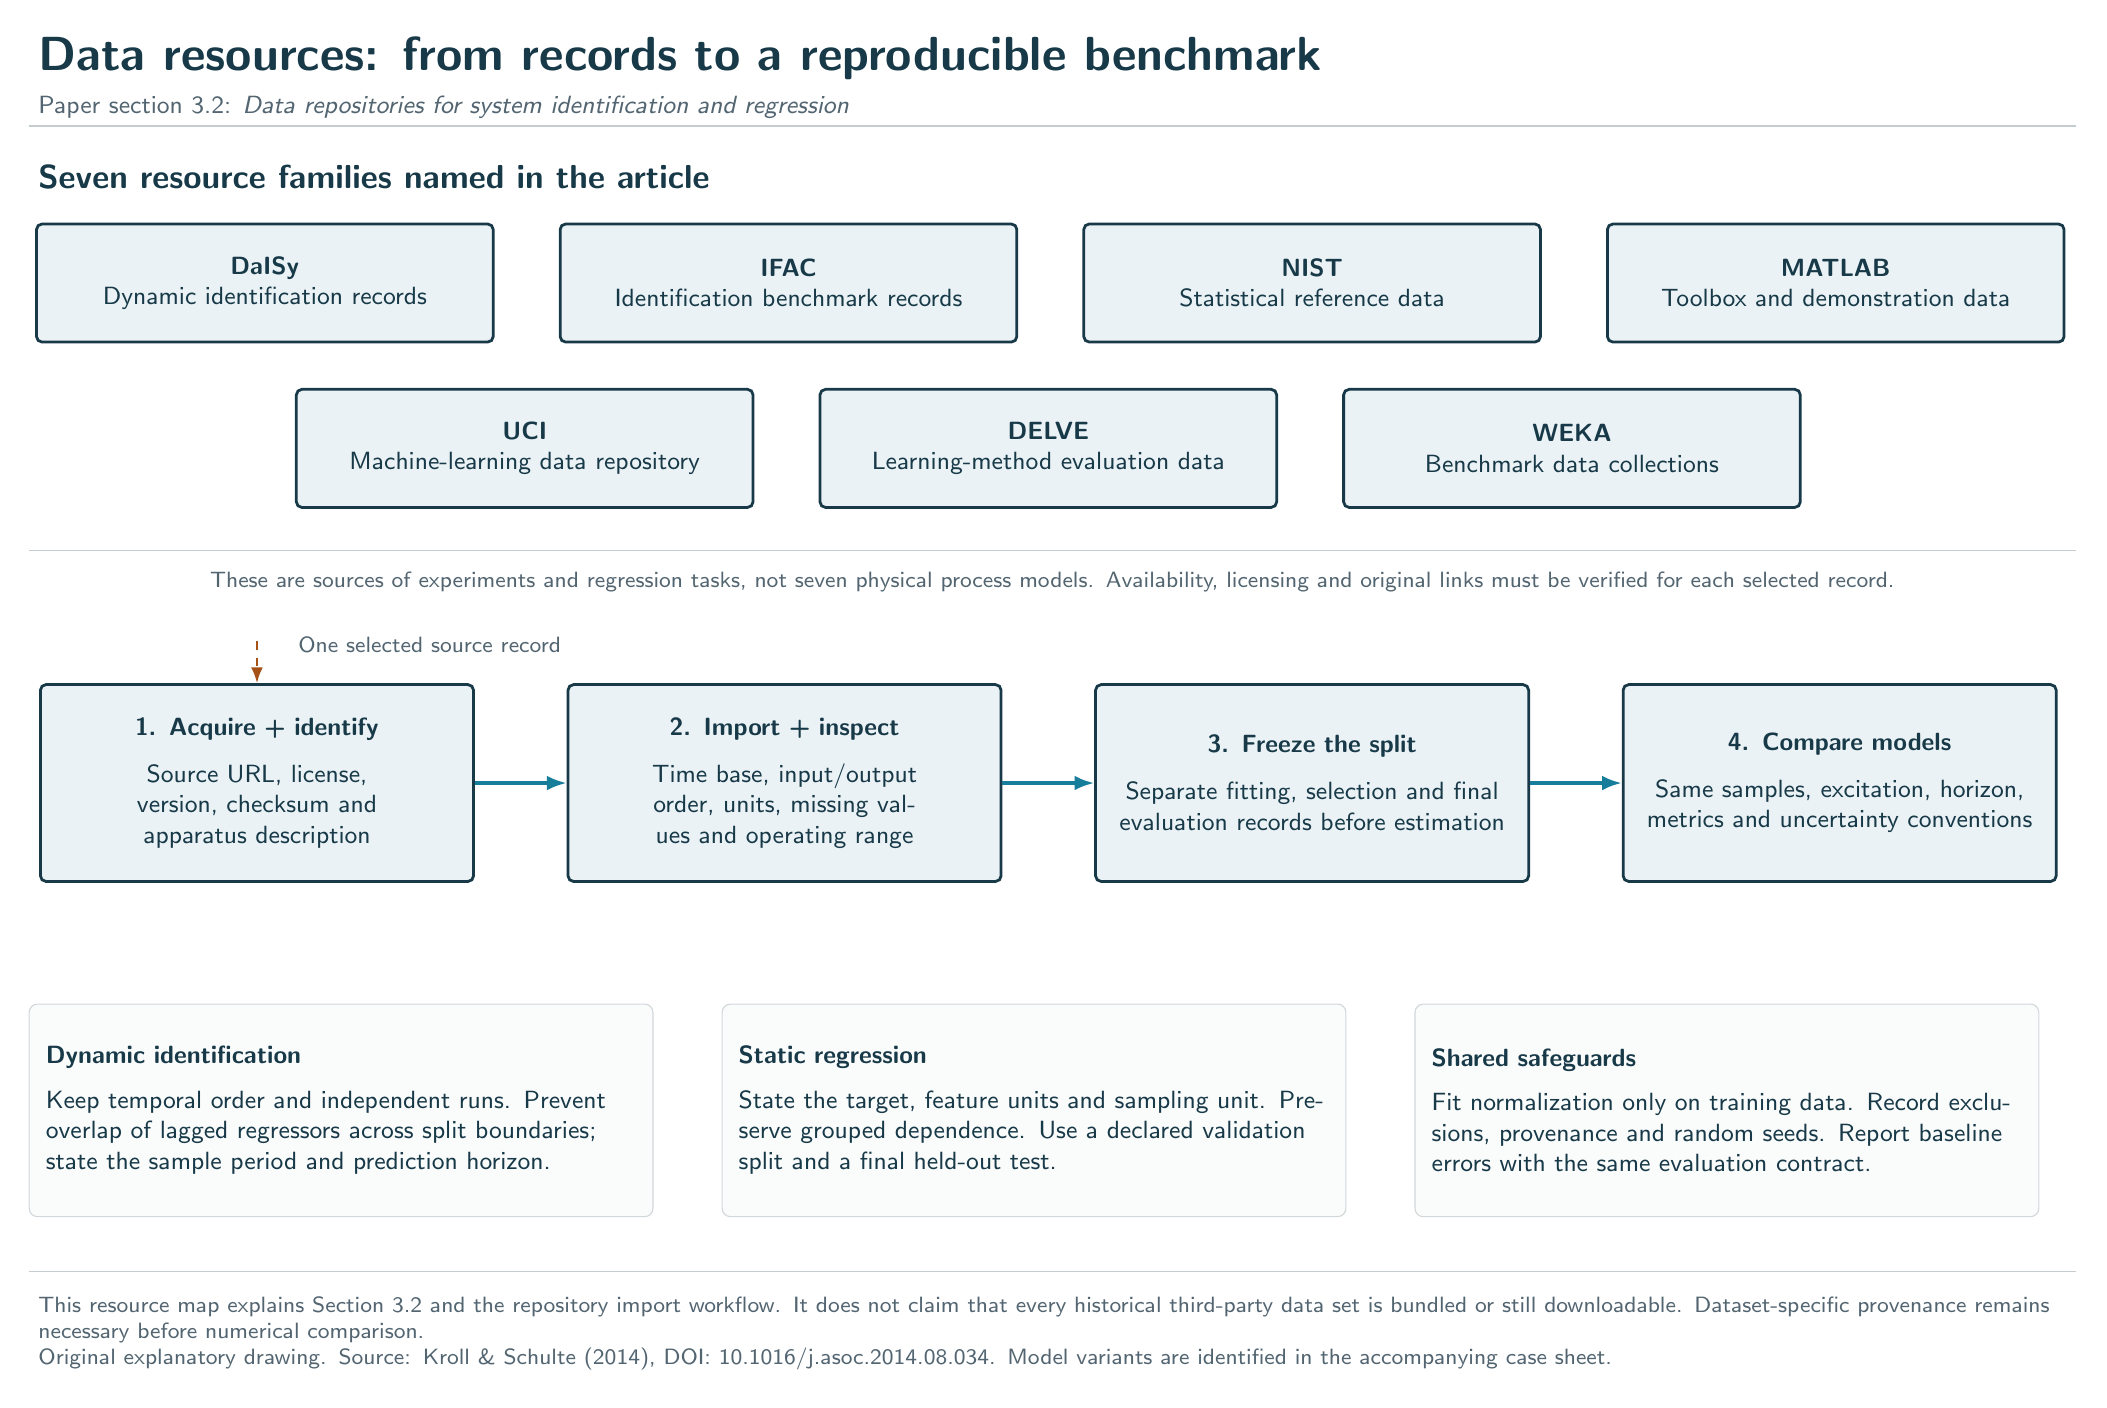
\begin{tikzpicture}[x=1cm,y=1cm]
\atlasheader{Data resources: from records to a reproducible benchmark}{3.2}{Data repositories for system identification and regression}
\node[anchor=west,font=\sffamily\bfseries\large] at (0,-1.9) {Seven resource families named in the article};
\node[box,minimum width=5.8cm,minimum height=1.5cm] (daisy) at (3,-3.25) {\textbf{DaISy}\\Dynamic identification records};
\node[box,minimum width=5.8cm,minimum height=1.5cm] (ifac) at (9.65,-3.25) {\textbf{IFAC}\\Identification benchmark records};
\node[box,minimum width=5.8cm,minimum height=1.5cm] (nist) at (16.3,-3.25) {\textbf{NIST}\\Statistical reference data};
\node[box,minimum width=5.8cm,minimum height=1.5cm] (matlab) at (22.95,-3.25) {\textbf{MATLAB}\\Toolbox and demonstration data};
\node[box,minimum width=5.8cm,minimum height=1.5cm] (uci) at (6.3,-5.35) {\textbf{UCI}\\Machine-learning data repository};
\node[box,minimum width=5.8cm,minimum height=1.5cm] (delve) at (12.95,-5.35) {\textbf{DELVE}\\Learning-method evaluation data};
\node[box,minimum width=5.8cm,minimum height=1.5cm] (weka) at (19.6,-5.35) {\textbf{WEKA}\\Benchmark data collections};
\draw[ink!25] (0,-6.65)--(26,-6.65);
\node[anchor=north,annotation,text width=24.5cm,align=center] at (13,-6.8)
 {These are sources of experiments and regression tasks, not seven physical process models. Availability, licensing and original links must be verified for each selected record.};

\node[box,minimum width=5.5cm,minimum height=2.5cm,text width=4.9cm] (acquire) at (2.9,-9.6)
 {\textbf{1. Acquire + identify}\\[6pt]Source URL, license, version, checksum and apparatus description};
\node[box,minimum width=5.5cm,minimum height=2.5cm,text width=4.9cm] (contract) at (9.6,-9.6)
 {\textbf{2. Import + inspect}\\[6pt]Time base, input/output order, units, missing values and operating range};
\node[box,minimum width=5.5cm,minimum height=2.5cm,text width=4.9cm] (split) at (16.3,-9.6)
 {\textbf{3. Freeze the split}\\[6pt]Separate fitting, selection and final evaluation records before estimation};
\node[box,minimum width=5.5cm,minimum height=2.5cm,text width=4.9cm] (score) at (23,-9.6)
 {\textbf{4. Compare models}\\[6pt]Same samples, excitation, horizon, metrics and uncertainty conventions};
\draw[process] (acquire.east)--(contract.west);
\draw[process] (contract.east)--(split.west);
\draw[process] (split.east)--(score.west);
\draw[signal] (2.9,-7.8)--(acquire.north);
\node[anchor=west,annotation] at (3.3,-7.85) {One selected source record};

\node[panel,anchor=north west,text width=7.5cm,minimum height=2.7cm,align=left] at (0,-12.4)
 {\textbf{Dynamic identification}\\[5pt]
 Keep temporal order and independent runs. Prevent overlap of lagged regressors across split boundaries; state the sample period and prediction horizon.};
\node[panel,anchor=north west,text width=7.5cm,minimum height=2.7cm,align=left] at (8.8,-12.4)
 {\textbf{Static regression}\\[5pt]
 State the target, feature units and sampling unit. Preserve grouped dependence. Use a declared validation split and a final held-out test.};
\node[panel,anchor=north west,text width=7.5cm,minimum height=2.7cm,align=left] at (17.6,-12.4)
 {\textbf{Shared safeguards}\\[5pt]
 Fit normalization only on training data. Record exclusions, provenance and random seeds. Report baseline errors with the same evaluation contract.};
\atlasfooter{This resource map explains Section 3.2 and the repository import workflow. It does not claim that every historical third-party data set is bundled or still downloadable. Dataset-specific provenance remains necessary before numerical comparison.}
\end{tikzpicture}
\end{document}
